\documentclass[11pt]{article}

\usepackage[portuguese]{babel}
\usepackage[utf8]{inputenc}
\usepackage{amsmath}
\usepackage{graphicx}
\usepackage{float}
\usepackage{subfig}
\usepackage{fixltx2e}
\usepackage[bottom]{footmisc}
\usepackage{color}
\usepackage[usenames,dvipsnames]{xcolor}
\usepackage[font=footnotesize]{caption}
\numberwithin{equation}{section}

\linespread{1.3}
\usepackage{indentfirst}
\usepackage[top=2cm, bottom=2cm, right=2.5cm, left=2.5cm]{geometry}
\addto\captionsportuguese{\renewcommand{\contentsname}{Índice}}

\begin{document}

\begin{titlepage}
\begin{center}

\hfill \break
\hfill \break


\includegraphics[width=0.3\textwidth]{./logo}~\\[1cm]

\textsc{\LARGE Instituto Superior Técnico}\\[0.25cm]
\textsc{\Large Mestrado Integrado em Engenharia Electrotécnica e de Computadores}\\[1.8cm]
\textsc{\huge Sistemas Integrados Analógicos}\\[0.25cm]

{\huge \bfseries Projecto de Alto Nível de um ADC e DAC \\[1cm]}

\begin{tabular}{ l l }
Maria Margarida Dias dos Reis & \hspace{2mm} n.º 73099 \\
Nuno Miguel Rodrigues Machado & \hspace{2mm} n.º 74236

\end{tabular}

\vfill

{\large Lisboa, 16 de Março de 2015} 

\end{center}
\end{titlepage}

\pagenumbering{gobble}
\clearpage

\tableofcontents
\pagebreak

\clearpage
\pagenumbering{arabic}

\section{Introdução}

Com este trabalho laboratorial pretende-se introduzir o \textit{software} Cadence, projectando um conversor AD/DA de alto nível. Analisando os conversores analógico-digitais (ADC) pode-se melhor compreender o conceito de \textit{Fast Fourier Transform} (FFT), e a maneira como pode ser aplicada para medir parâmetros dos ADC, como a SINAD e o ENOB. Pretende-se também estudar o efeito de aplicar diversas janelas sobre a FFT.

\section{Introdução Teórica}
\subsection{Conversores A/D e Conversores D/A}

Começando por analisar os conversores analógico-digitais, as arquitecturas que os permitem podem ser divididas em três categorias: baixa-a-média velocidade, média velocidade e alta velocidade. O ADC utilizado neste trabalho é de aproximações sucessivas (SAR), sendo de média velocidade e exactidão. 

Os conversores deste tipo estão entre os mais populares para realizar ADCs devido à sua versatilidade - conseguem efectuar conversões rápidas ou podem ser utilizados para que haja uma maior exactidão, operando a baixa potência nos dois casos. Este conjunto de características deriva de, no caso mais simples, o conversor necessitar apenas de um só comparador, um banco de condensadores com interruptores e pouca lógica de controlo digital. Na figura abaixo está esquematizado o circuito referido.

\begin{figure}[h]
	\centering
	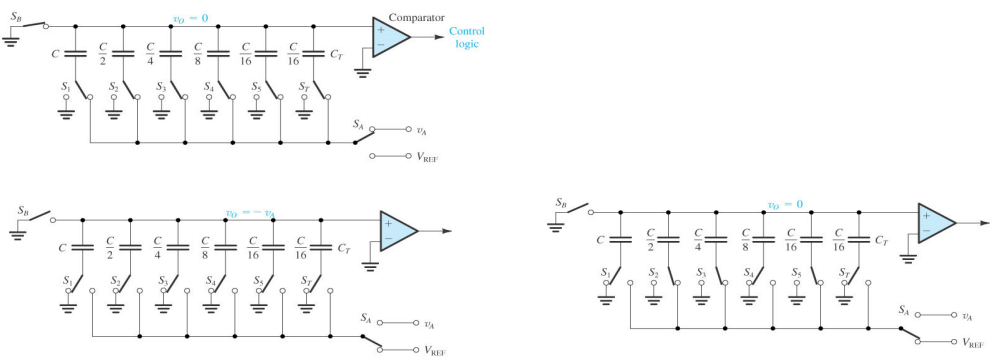
\includegraphics[keepaspectratio=true, scale=0.45]{./teoricas/SAR_1}
	\caption{ADC construído com uma arquitectura de aproximações sucessivas.}
	\vspace{-0.8em}
\end{figure}

OS ADCs de aproximações sucessivas têm por base o algoritmo de procura conhecido como ``procura binária'', onde os dados podem ser calculados em $N$ passos, para um conjunto de dados organizados de tamanho $2^N$. Assim, o conversor aplica o algoritmo para determinar a palavra digital mais próxima que corresponde ao sinal de entrada. Isto implica que são necessários $N$ ciclos de relógio para completar uma conversão de $N$ \textit{bits}.

O diagrama de blocos de um ADC unipolar de aproximações sucessivas que utiliza também um DAC é apresentado de seguida.

\begin{figure}[h]
	\centering
	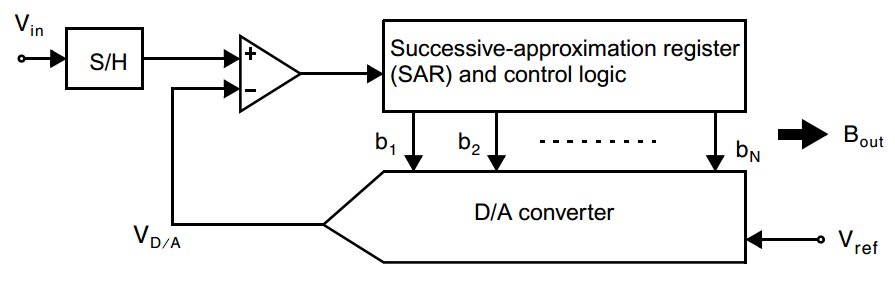
\includegraphics[keepaspectratio=true, scale=0.30]{./teoricas/SAR_2}
	\caption{ADC construído com uma arquitectura de aproximações sucessivas.}
	\vspace{-0.8em}
\end{figure}

O princípio de funcionamento 

\subsection{SNR}
\subsection{SINAD e ENOB}
\subsection{Janela Rectangular, Janela de Hamming e Janela de Blackman-Harris}

\end{document}